\documentclass[letter, 10pt]{article}
\usepackage[top=2.5cm, bottom=2cm, left=2cm, right=2cm]{geometry}
\usepackage[utf8x]{inputenc}
\usepackage[spanish]{babel}
\usepackage{amsfonts}
\usepackage{amsmath}
\usepackage{graphicx}
\usepackage{listings}
\lstset{language=Matlab}
\lstset{tabsize=2}
\lstset{flexiblecolumns=true}

\title{Laboratorio $\#$ 3\\
       Computaci\'on Cient\'ifica II\\}
\author{\bf Alumno: Diego Villouta Fredes\\
\bf Rol: 2773019-1}

\begin{document}

\begin{titlepage}
\maketitle
\thispagestyle{empty}
\end{titlepage}

\tableofcontents

\newpage

\section{ Introducci\'on }

\begin{itemize}
\item En el \'area de m\'etodos num\'ericos y de la computaci\'on cient\'ifica en general, es com\'un trabajar con ecuaciones diferenciales, debido a las aplicaciones que pueden tener estas al usarlas para modelar fenomenos de la f\'isica, como en este caso ser\'ia una ecuaci\'on de calor.\\
\item Mediante el uso de la poderosa herramienta matem\'atica MatLab, se busca resolver una ecuaci\'on de este tipo aplicando el m\'etodo de Forward Difference para ecuaciones parab\'olicas.\\
\end{itemize}

\section{ Objetivos }

\begin{itemize}
\item Implementar la resoluci\'on de la ecuaci\'on de calor en una barra, de modo de obtener su aproximaci\'on mediante ecuaciones diferenciales parciales bajo diferentes condiciones de borde, en este caso corresponde a una ecuaci\'on parab\'olica.\\
\item Generar una soluci\'on para una ecuaci\'on diferencial utilizando el m\'etodo de Forward Difference.\\
\item Utilizar la herramienta MatLab u Octave para desarrollar el laboratorio.\\
\item Realizar gr\'aficos comparativos de como var\'ian las soluciones con respecto al tiempo.
\end{itemize}

\newpage

\section{ Desarrollo }

\subsection{Ejercicio 1}
\begin{itemize}
\item Se pide programar la funci\'on eqHeatFD.m, la cual fue implementada siguiendo la idea del Pseudo-c\'odigo adjunto, de la siguiente forma:

\begin{lstlisting}
%Recibe como inputs el largo L de la barra, el intervalo de distancia entre puntos h, intervalo de tiempo k,el factor
%alfa y el numero maximo de iteraciones a considerar como condicion de termino para el problema.

function [result] = eqHeatFD(L, h, k, alfa, MAX_ITER)
%Valores iniciales eqHeatFD(1,0.01,0.00000001,1,5000)	
	result = [];
	m = L/h;

%Se genera la particion de m intervalos con m+1 valores, correspondientes a los X_i a evaluar.
	X = linspace(0,L,m+1);
	u_0 = zeros(1,m+1);
	u_j = [];

%Se evaluan los X_i en la funcion de la condicion inicial para generar el vector U_0 inicial.
%De este vector, por condicion de borde, el primer y ultimo valor deben ser cero, por lo que no se evaluan
%en la funcion.
	for i = 2:m,
		u_0(i) = (exp(2*X(i)))*sin(X(i))*cos(X(i));
	end

%Se crea la matriz tridiagonal A.
	A = zeros(m+1,m+1);
	lambda = ((alfa^2)*k)/(h^2);
	dif = 1-(2*lambda);
	
	for i = 1:m+1,
		if i == 1
			A(1,i) = dif;
			A(1,i+1) = lambda;
		elseif i == m+1
			A(i,i) = dif;
			A(i,i-1) = lambda;
		else
			A(i,i) = dif;
			A(i,i-1) = lambda;
			A(i,i+1) = lambda;
	end
	
	u_ant = u_0;

%Se ejecuta lo que aparece en el pseudo-codigo desde la linea 5 hasta la linea 12.
	for iter = 1:MAX_ITER,
		u_j = A*u_ant';

%Se aplica la condicion de borde donde el primer y ultimo elemento de u_j deben ser cero.
		u_j(1) = 0;
		u_j(m+1) = 0;

		u_j2 = u_j';
		
		diferencia = u_j' - u_ant;
		
%Se agregan vectores u_j generados a una matriz de resultados, para ser usada al momento de graficar.
		result(:,iter) = u_ant;
		
		u_ant = u_j2;		
		
%Condicion de termino del algoritmo. Si la diferencia entre dos vectores U_j consecutivos es menor
%a cierta cota, se almacena el ultimo vector generado y se detiene el algoritmo.
		if max(abs(diferencia)) <= (1.1*10^(-4))
			result(:,iter) = u_ant;
			break
		end
	end
end
\end{lstlisting}
\end{itemize}

\subsection{Ejercicio 2}
\begin{itemize}
\item Se pide graficar el comportamiento de la funci\'on U para los puntos obtenidos anteriormente. El c\'odigo a continuaci\'on, cabe destacar lo breve que es ya que solo recibe datos y los grafica:

\begin{lstlisting}
%Recibe el parametro MAX_ITER el cual segun el laboratorio debe ser 5000, y corresponde al numero
%maximo de iteraciones del algoritmo antes de detenerse.

function [] = surfaceDataTime(MAX_ITER)
	mesh(eqHeatFD(1,0.01,0.00000001,1,MAX_ITER))
end
\end{lstlisting} 

\item A continuaci\'on, el gr\'afico:

\begin{center}
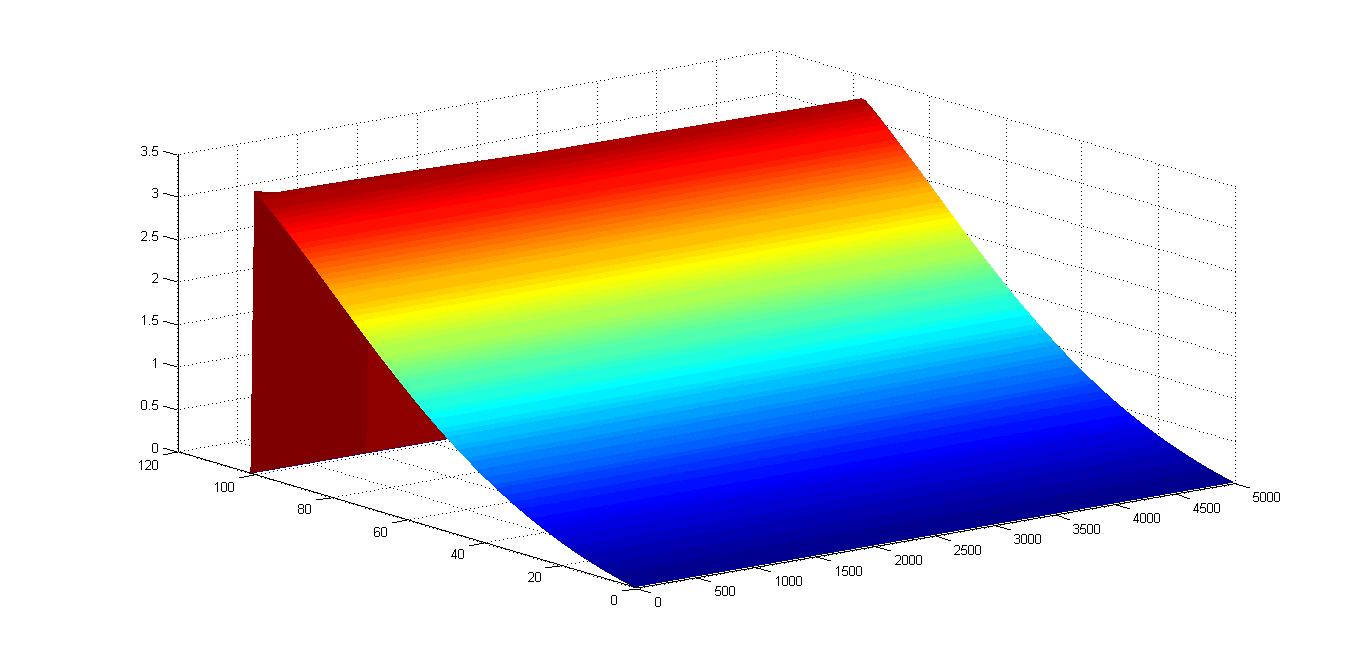
\includegraphics[width=18cm]{grafico1.png}
\end{center}

\end{itemize}

\subsection{Ejercicio 3}
\begin{itemize}
\item Se pide graficar el comportamiento de la funci\'on U a lo largo de un numero de iteraciones $t=20$ dentro de la porci\'on de la barra $[0;0,5][m]$. El c\'odigo a continuaci\'on, es bastante breve ya que solo recibe datos y los grafica:

\begin{lstlisting}
%Recibe como parametros el largo de la barra a utilizar y el numero de iteraciones.
%Para este caso son L = 0.5, MAX_ITER = 20.

function [] = surfaceDataInterval(L, MAX_ITER)
	result = eqHeatFD(L, 0.01, 0.00000001, 1, MAX_ITER);
	plot(result')
end
\end{lstlisting}

\item  A continuaci\'on el gr\'afico:

\begin{center}
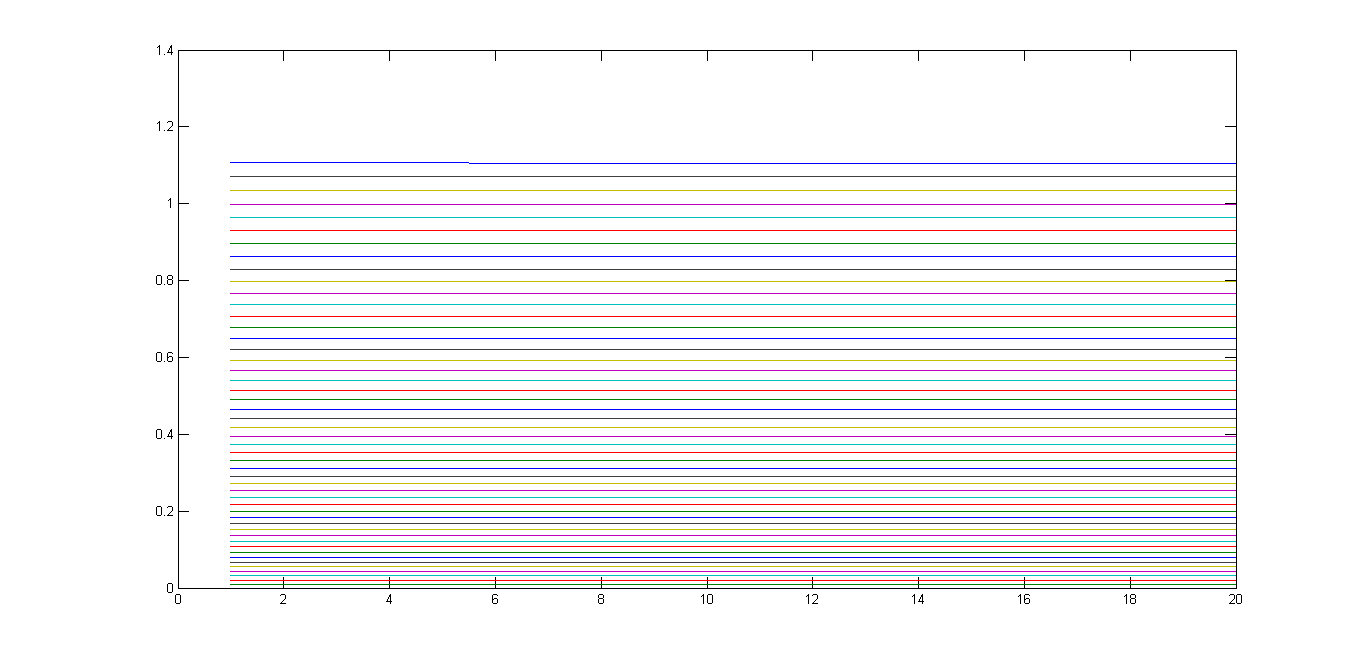
\includegraphics[width=18cm]{grafico2.png}
\end{center}
\end{itemize}

\newpage

\section{ Conclusiones }
\begin{itemize}
\item Se puede observar que el comportamiento de las temperaturas a lo largo de la barra, se mantienen constantes a travez del tiempo. Lo m\'as probable es que al agrandar los valores de h y k, se vean m\'as variaciones en las temperaturas, o al ejecutar un n\'umero mayor de iteraciones.
\item El pseudo-c\'odigo entregado, se comprob\'o que funciona correctamente, sin embargo se le podr\'ian agregar detalles de manera de mejorar su funcionamiento, tales como generar una matriz que devuelva todos los vectores generados por iteraci\'on, m\'as detalle sobre como crear el vector $u_0$ y sobre el porque de las dimensiones de la matriz A.
\end{itemize}

\section{ Anexos }
\begin{itemize}
\item Cualquier input necesario para el laboratorio, se incluye dentro de las mismas funciones, y se encuentran ademas en los enunciados del mismo.
\end{itemize}

\end{document}